\documentclass[tikz,border=0.2cm]{standalone}
\usepackage{tikz}
\usetikzlibrary{backgrounds}
\begin{document}
    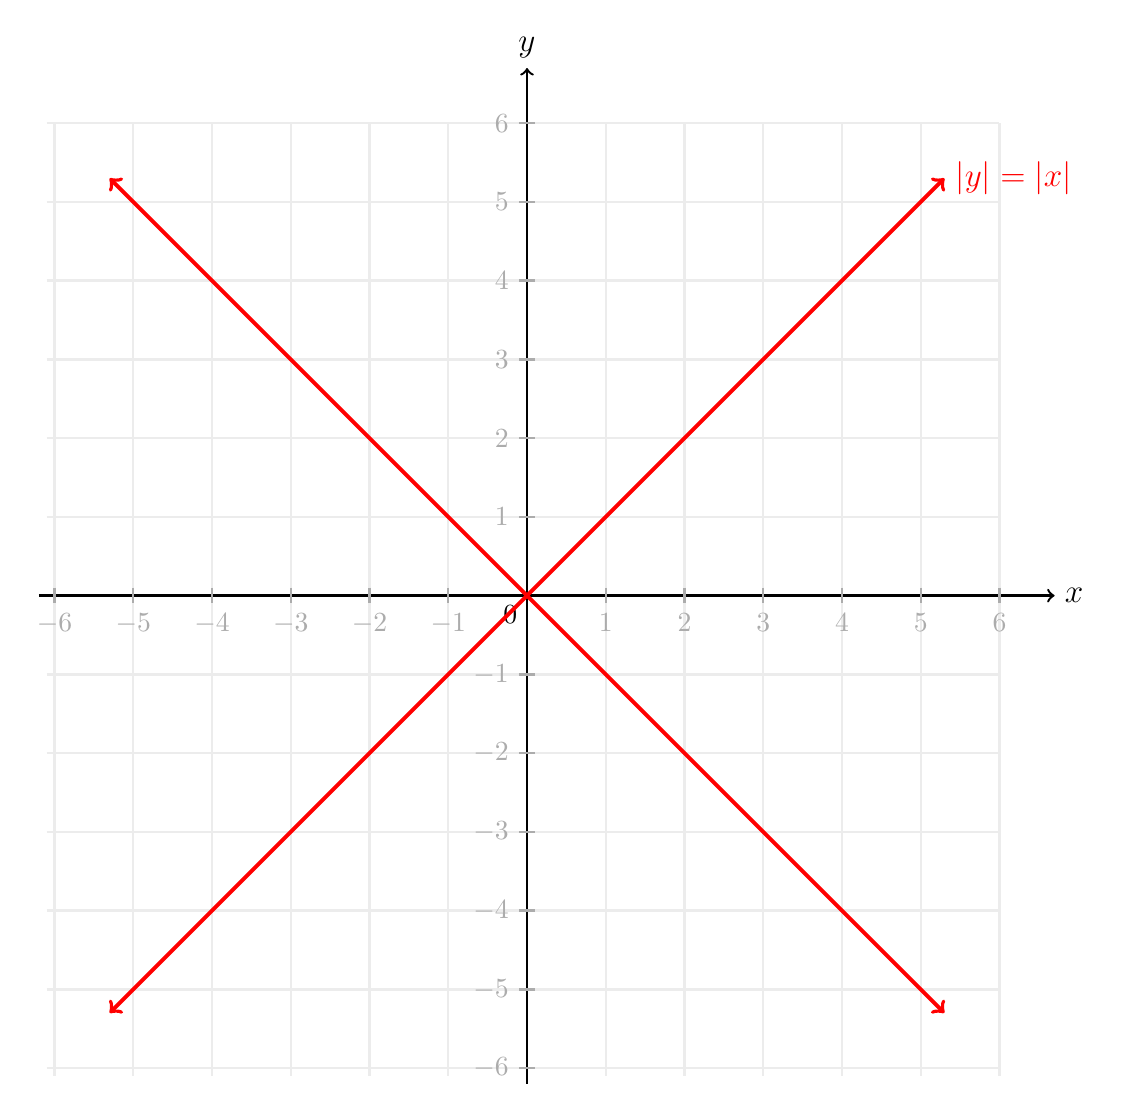
\begin{tikzpicture}[background rectangle/.style={fill=white},]
        \draw[line width=0.3mm,color=gray!15,step=1] (-6.1,-6.1) grid (6,6);
        \draw[line width=0.3mm,->] (-6.2,0) -- (6.7,0) node[font=\large,right] {$x$};
        \draw[line width=0.3mm,->] (0,-6.2) -- (0,6.7) node[font=\large,above] {$y$};
        \coordinate [label=below left:0] (a) at (0,0);
        \foreach \i in {-6,...,-2,-1,1,2,...,6}
        \draw[line width=0.3mm,gray!65] (\i,.1)--(\i,-.1) node[below] {$\i$};
        \foreach \i in {-6,...,-2,-1,1,2,...,6}
        \draw[line width=0.3mm,gray!65] (.1,\i)--(-.1,\i) node[left] {$\i$};

       \draw[line width=0.5mm,  red, <->] (-5.3,-5.3) -- (5.3,5.3) node[font=\large,right] {$|y| = |x|$};
       \draw[line width=0.5mm,  red,  <->] (-5.3,5.3) -- (5.3,-5.3);

%\node[font=\large,align=center] {x\\y}

    \end{tikzpicture}
\end{document}